\section{Case study}

To show the functionality and applicability of the automatic domain decomposition library a few case studies were carried out.
This chapter and the following sections will outline each case study and the corresponding experimental results.

The base implementation of each test case was provided by Stefano Ubbiali written in Python and using GT4Py stencils.

\subsection{Case 1: Burger's equation}
Burger's equation is a well-known nonlinear partial differential equation.
It is widely used to test numerical schemes since it has analytical solutions for a set of initial conditions.
Burger's equation can be used to model various physical phenomena.
Most commonly it is used as a model for traffic flow or shock waves in a fluid.

\subsubsection{Case description}

The two-dimensional, viscid Burger's equation is given by the following system of equations as described in \citet{zhao2011new}:

\begin{equation}
\begin{split}
\pdv{u}{t} + u \pdv{u}{x} + v \pdv{u}{y} = \varepsilon \left( \pdv{^2 u}{x^2} + \pdv{^2 u}{y^2} \right) \\
\pdv{v}{t} + u \pdv{v}{x} + v \pdv{v}{y} = \varepsilon \left( \pdv{^2 v}{x^2} + \pdv{^2 v}{y^2} \right) \\
\text{with } \left(x, y, t\right) \in D \times \left(0,T\right]
\end{split}
\end{equation}

These two equations characterize the Burger equation as set of equations for the velocity in x and y direction.
Both equations describe two parts.
On the left hand side of the equation the advection of the velocity itself.
On the right hand side of the equation the diffusion caused by viscosity.

To complete the full description of the Burger equation the initial and boundary conditions are generally given by the following equations:

\begin{equation}
\begin{split}
\text{Initial conditions: } \\
u\left(x, y, 0\right) = u_0\left(x, y\right), \left(x, y\right) \in D \\
v\left(x, y, 0\right) = v_0\left(x, y\right), \left(x, y\right) \in D \\
\text{Boundary conditions: } \\
u\left(x, y, t\right) = f\left(x, y, t\right), \left(x, y, t\right) \in \partial D \times \left(0, T\right] \\
v\left(x, y, t\right) = g\left(x, y, t\right), \left(x, y, t\right) \in \partial D \times \left(0, T\right]
\end{split}
\end{equation}

% TODO FOOTNOTE CHECK CORRECT NUMBERING

\paragraph{Shankar conditions:}

The first set of initial and boundary conditions are the ones used by Shankar. \footnote{https://ch.mathworks.com/matlabcentral/fileexchange/38087-burgers-equation-in-1d-and-2d}

The following equations describe the Shankar test case fully and fig. \ref{fig:shankar_ic1} and fig. \ref{fig:shankar_ic2} visualizes the initial condition.

\begin{equation}
\begin{split}
\text{\textbf{Boundary conditions: }} \\
f\left(x, y, t\right) = 0 \\
g\left(x, y, t\right) = 0 \\
\\
\text{\textbf{Other parameters: }} \\
\text{Viscosity: } \varepsilon = 0.01
\end{split}
\quad
\begin{split}
\text{\textbf{Initial conditions: }} \\
u_0\left(x, y\right) = \begin{cases}
0, \text{ in } \left[0.5, 1.0\right] \times \left[0.5, 1.0\right] \\
1, \text{ otherwise}
\end{cases}
\\
v_0\left(x, y\right) =  \begin{cases}
1, \text{ in } \left[0.5, 1.0\right] \times \left[0.5, 1.0\right] \\
0, \text{ otherwise}
\end{cases}
\\
\text{\textbf{Domain: }} \\
D = \left[0,2\right] \times \left[0,2\right] \\
T = 0.6 \\
\end{split}
\end{equation}

\begin{figure}
\centering
\begin{subfigure}{.5\textwidth}
  \centering
  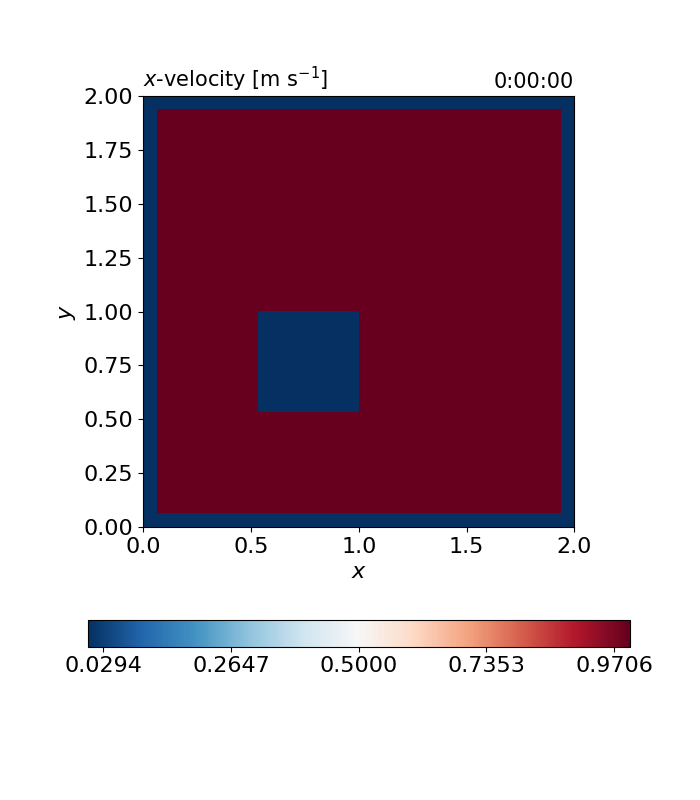
\includegraphics[width=1.1\linewidth]{test_shankar_forward_backward_field_u_at_0.png}
  \caption{X-velocity initial condition.}
  \label{fig:shankar_ic1}
\end{subfigure}%
\begin{subfigure}{.5\textwidth}
  \centering
  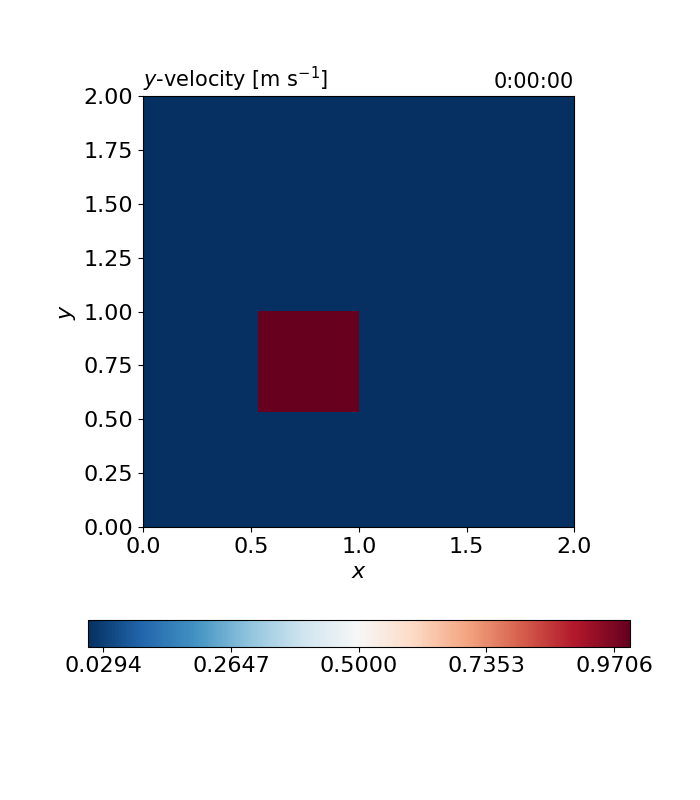
\includegraphics[width=1.1\linewidth]{test_shankar_forward_backward_field_v_at_0.png}
  \caption{Y-Velocity initial condition.}
  \label{fig:shankar_ic2}
\end{subfigure}
\caption{Initial condition for the Shankar test case.}
\label{fig:shankar_ic}
\end{figure}


\paragraph{Zhao conditions:}

The second set of initial and boundary conditions are the same as used as example 1 in \citet{zhao2011new}:

\begin{equation}
\begin{split}
\text{\textbf{Boundary conditions: }} \\
f\left(x, y, t\right) = \begin{cases}
-2 \varepsilon \pi \exp^{-5 \pi^2 \varepsilon t} \sin\left(\pi y\right) \text{, for } x = 0, y \in \left[0, 1\right] \\
-2 \varepsilon \pi \exp^{-5 \pi^2 \varepsilon t} \sin\left(\pi y\right) \text{, for } x = 1, y \in \left[0, 1\right] \\
0 \text{, for } x \in \left[0, 1\right], y = 0 \\
0 \text{, for } x \in \left[0, 1\right], y = 1 \\
\end{cases}
\\
g\left(x, y, t\right) = \begin{cases}
0 \text{, for } x = 0, y \in \left[0, 1\right] \\
0 \text{, for } x = 1, y \in \left[0, 1\right] \\
-\varepsilon \pi \exp^{-5 \pi^2 \varepsilon t} \sin\left(2 \pi x\right) \text{, for } x \in \left[0, 1\right], y = 0 \\
\varepsilon \pi \exp^{-5 \pi^2 \varepsilon t} \sin\left(2 \pi x\right) \text{, for } x \in \left[0, 1\right], y = 1 \\
\end{cases}
\\
\text{\textbf{Other parameters: }} \\
\text{Viscosity: } \varepsilon = 0.01
\end{split}
\quad
\begin{split}
\text{\textbf{Initial conditions: }} \\
u_0\left(x, y\right) = \frac{-4 \varepsilon \pi \cos \left(2 \pi x\right) \sin \left(\pi y\right)}{2 + \sin \left(2 \pi x \right) \sin \left(\pi y\right)}
\\
v_0\left(x, y\right) = \frac{-2 \varepsilon \pi \sin \left(2 \pi x\right) \cos \left(\pi y\right)}{2 + \sin \left(2 \pi x \right) \sin \left(\pi y\right)}
\\
\text{\textbf{Domain: }} \\
D = \left[0,1\right] \times \left[0,1\right] \\
T = 1 \\
\end{split}
\end{equation}

\begin{figure}
\centering
\begin{subfigure}{.5\textwidth}
  \centering
  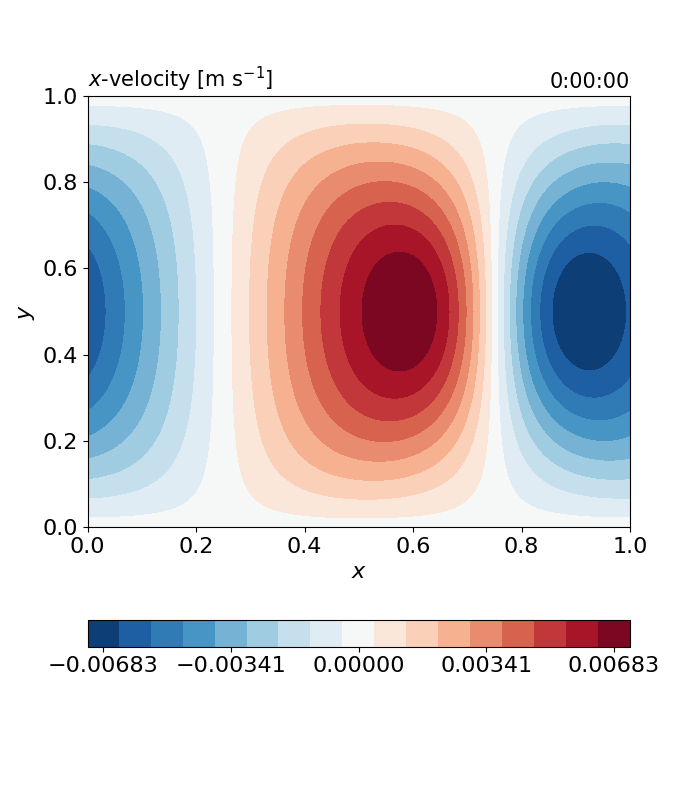
\includegraphics[width=1.1\linewidth]{test_zhao_forward_backward_field_u_at_0.png}
  \caption{X-velocity initial condition.}
  \label{fig:zhao_ic1}
\end{subfigure}%
\begin{subfigure}{.5\textwidth}
  \centering
  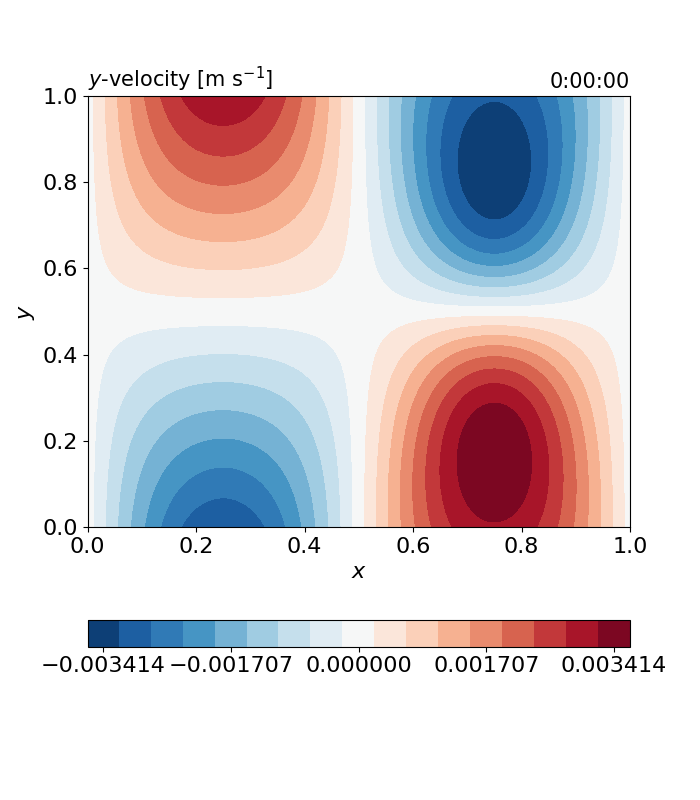
\includegraphics[width=1.1\linewidth]{test_zhao_forward_backward_field_v_at_0.png}
  \caption{Y-Velocity initial condition.}
  \label{fig:zhao_ic2}
\end{subfigure}
\caption{Initial condition for the Zhao test case.}
\label{fig:zhao_ic}
\end{figure}

Notable about this set of initial and boundary condition is that they have exact solutions.
The exact solutions as provided in \citet{zhao2011new} are:
\\
\begin{equation}
\begin{split}
u\left(x,y,t\right) = -2\varepsilon \frac{2 \pi \exp^{-5 \pi^2 \varepsilon t} \cos\left(2 \pi x\right) \sin\left(\pi y\right)}{2 + \exp^{-5 \pi^2 \varepsilon t}\sin\left(2 \pi x\right) \sin\left(\pi y\right)}
\\
v\left(x,y,t\right) = -2\varepsilon \frac{\pi \exp^{-5 \pi^2 \varepsilon t} \sin\left(2 \pi x\right) \cos\left(\pi y\right)}{2 + \exp^{-5 \pi^2 \varepsilon t}\sin\left(2 \pi x\right) \sin\left(\pi y\right)}
\end{split}
\end{equation}

\subsubsection{Implementation details}
Both the Shankar and Zhao conditions can be solved using different numerical stencils for the computation.
To show some variance and flexibility three stencils can be used to solve the test case.

The forward-backward stencil combines forward finite differences to compute the time derivatives with backward finite differences to compute the first-order space derivatives and a second-order centered scheme to compute the second-order derivatives.
See fig. \ref{fig:fb_stencil} for a visual representation of this stencil.

The other two stencil are called upwind schemes, since they use the values only from the direction the velocity is coming from.
The first-order upwind scheme uses the directly neighboring grid points like the forward-backward stencil.
The difference is that only the values from upwind are used in the actual computation for the next value.
See fig. \ref{fig:upwind_stencil} for a visual representation of this stencil.

The third-order upwind stencil needs two neighboring grid points in each direction to increase the accuracy of the approximated space derivative.
See fig. \ref{fig:upwind_third_stencil} for a visual representation of this stencil.

\begin{figure}[!htbp]
\centering
\begin{subfigure}{.3\textwidth}
  \centering
  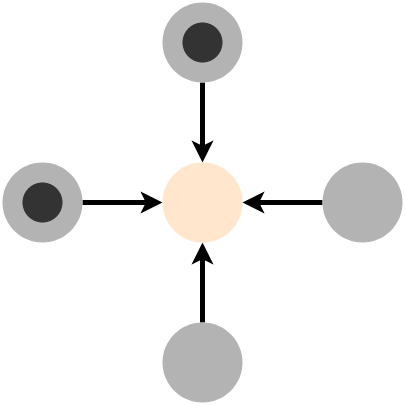
\includegraphics[width=0.8\linewidth]{fb_stencil.png}
  \caption{Forward-backward}
  \label{fig:fb_stencil}
\end{subfigure}%
\begin{subfigure}{.3\textwidth}
  \centering
  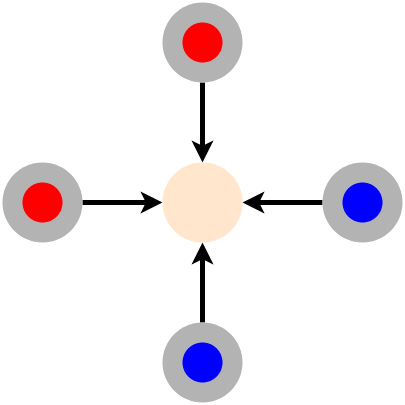
\includegraphics[width=0.8\linewidth]{upwind.png}
  \caption{Upwind first order}
  \label{fig:upwind_stencil}
\end{subfigure}
\begin{subfigure}{.3\textwidth}
  \centering
  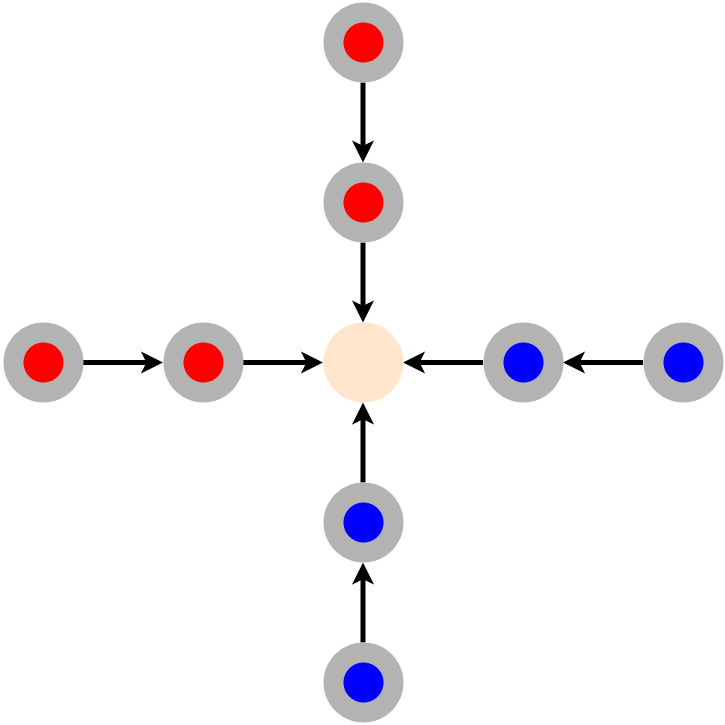
\includegraphics[width=0.8\linewidth]{upwind_third.png}
  \caption{Upwind third order}
  \label{fig:upwind_third_stencil}
\end{subfigure}
\caption{Schema for three possible stencils for the Burger's equation. The large gray circle indicate the grid points necessary for the computation of the Laplacian for the diffusion part of the Burger's equation. The small dark gray circle indicate grid points necessary for the backward finite difference. The red and blue small circles indicate grid points needed for the upwind computations in the case of positive velocity or negative velocity respectively.}
\label{fig:burger_stencils}
\end{figure}


\subsubsection{Experimental setup}

\subsubsection{Experimental results}


\subsection{Case 2: Shallow water equation}

\subsubsection{Case description}

\subsubsection{Implementation details}

\subsubsection{Experimental setup}

\subsubsection{Experimental results}
